%--------------------
% Packages
% -------------------
\documentclass[11pt,a4paper]{article}
\usepackage[utf8x]{inputenc}
\usepackage[T1]{fontenc}
%\usepackage{gentium}
\usepackage{mathptmx} % Use Times Font


\usepackage[pdftex]{graphicx} % Required for including pictures
\usepackage[pdftex,linkcolor=black,pdfborder={0 0 0}]{hyperref} % Format links for pdf
\usepackage{calc} % To reset the counter in the document after title page
\usepackage{enumitem} % Includes lists

\frenchspacing % No double spacing between sentences
\linespread{1.2} % Set linespace
\usepackage[a4paper, lmargin=0.1666\paperwidth, rmargin=0.1666\paperwidth, tmargin=0.1111\paperheight, bmargin=0.1111\paperheight]{geometry} %margins
%\usepackage{parskip}

\usepackage[all]{nowidow} % Tries to remove widows
\usepackage[protrusion=true,expansion=true]{microtype} % Improves typography, load after fontpackage is selected

\usepackage{lipsum} % Used for inserting dummy 'Lorem ipsum' text into the template

\usepackage{plantuml}
\usepackage{float}
\usepackage{indentfirst}
\usepackage{subcaption}

\usepackage{etoolbox} % Adds '\clearpage' to every '\section command' (newpage).
\pretocmd{\section}{\clearpage}{}{} 

\newcommand{\inputdiagram}[1]{\input{Diagrams/out/#1}}
\newcommand{\textwidthdiagram}[2][1]{%
  \resizebox{#1\textwidth}{!}{\inputdiagram{#2}}%
}

%-----------------------
% Set pdf information and add title, fill in the fields
%-----------------------
\hypersetup{ 	
pdfsubject = {Program Systems Engineering},
pdftitle = {itssoover},
pdfauthor = {Ignas Časas, Mykolas Marius Budrys, Augustas Kniška}
}

%-----------------------
% Begin document
%-----------------------
\begin{document} %All text i dokumentet hamnar mellan dessa taggar, allt ovanför är formatering av dokumentet

\begin{titlepage}
    \centering
    % Remove page numbering from title
    \thispagestyle{empty}
    
    % University name
    {\Large VILNIAUS UNIVERSITETAS\\
    Matematikos ir informatikos fakultetas}\par
    
    \vspace{3cm} % vertical space
    
    % Title of the work
    {\Large 2\textsuperscript{nd} Laboratory Work}\par
    \vspace{0.5cm}
    {\Large \textbf{itssoover}}\par
    {\Large \textbf{Iteration, design and implementation}}\par
    
    \vspace{3cm}
    
    % Authors
    {\large
    Ignas Časas\\
    Mykolas Marius Budrys\\
    Augustas Kniška
    }\par
    
    \vspace{8cm}
    
    % Bottom of the page
    {\large
    Matematikos ir informatikos fakultetas\\
    Vilniaus universitetas\\
    Lietuva
    }\par
    
    \vfill

    \large 2025
    
\end{titlepage}

\section{Context}
 Some text and ideas are mentioned...

\section{Logical View}

\subsection*{Class Diagram}
    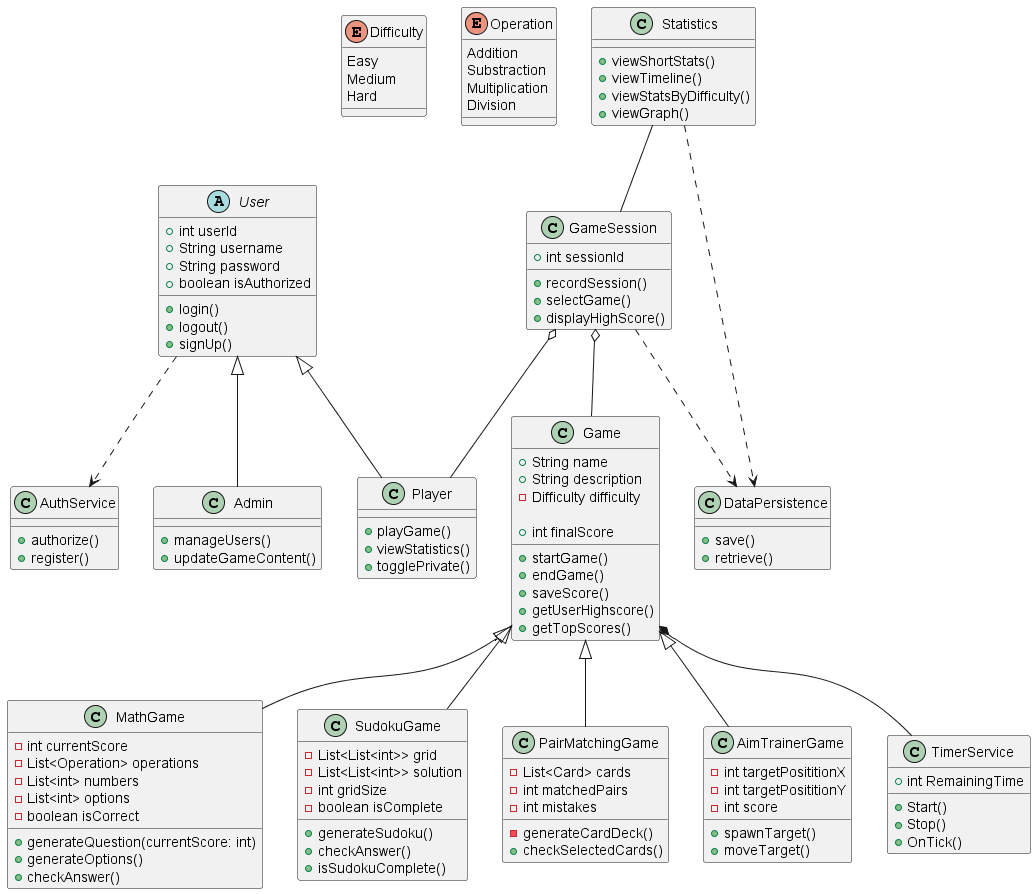
\includegraphics[width=\textwidth]{out/Diagrams/class_diagram/class_diagram.png}

\subsection*{State Diagram}
...State diagram

\section{Development View}

\subsection*{Package Diagram}
...Package diagram

\subsection*{Component Diagram}
...Component diagram

\section{Process View}

\subsection*{Sequence Diagram}
...Sequence diagram

\section{Physical View}
\begin{figure}[H]
    \centering
    \textwidthdiagram[0.8]{deployment_diagram.tex}
    \caption{Deployment diagram}
    \label{fig:deployment_diagram}
\end{figure}

Figure~\ref{fig:deployment_diagram} illustrates the architecture of the web application,
which consists of a client-side Blazor WebAssembly (WASM) front-end and a back-end hosted on an Azure server. The client browser executes the .NET WASM
runtime, running Client.dll as an executable. The backend operates in a Linux
environment within Azure, where the .NET runtime hosts Server.dll. Data is
persisted using an SQLite database. Communication between the client and
server occurs over HTTPS, ensuring secure data transmission. This design
enables a lightweight client while leveraging cloud infrastructure for
back-end processing and storage of user and game data.

\section{Use Case View}

\begin{figure}[H]
    \begin{minipage}[b]{0.48\textwidth}
        \centering
        \textwidthdiagram{use_case_account.tex}
        \caption{Account use case}
        \label{fig:use_case_account}
    \end{minipage}
    \hfil
    \begin{minipage}[b]{0.48\textwidth}
        \centering
        \textwidthdiagram{use_case_game_selection.tex}
        \caption{Game selection}
        \label{fig:use_case_game_selection}
    \end{minipage}
\end{figure}

Figure~\ref{fig:use_case_account} shows how players interact with the Account module.
Unauthenticated players can log in or sign up, while authenticated players can log out.

Figure~\ref{fig:use_case_game_selection} outlines two key actions: starting a game and
changing the difficulty level. This design ensures that players have direct
control over initiating gameplay and tailoring the challenge to their
preferences.

\begin{figure}[H]
    \centering
    \begin{minipage}[b]{0.48\textwidth}
        \textwidthdiagram{use_case_high_score.tex}
        \caption{High score module}
        \label{fig:use_case_high_score}
    \end{minipage}
    \hfil
    \begin{minipage}[b]{0.48\textwidth}
        \centering
        \textwidthdiagram{use_case_navigation.tex}
        \caption{Page navigation}
        \label{fig:use_case_navigation}
    \end{minipage}
\end{figure}

Figure~\ref{fig:use_case_high_score} details various ways for authenticated players to review game performance. Users
can view short game statistics, detailed graphs, timelines of past games, and
statistics filtered by difficulty. The module provides multiple perspectives to
help players track and analyze their performance.

Figure~\ref{fig:use_case_navigation} maps out the main paths for navigating through the website.
Players can easily switch between the home page (which doubles as the game
selection page), the account page, and the statistics page, ensuring a
user-friendly and integrated browsing experience.


\section{Traceability}

%\lipsum[1-3]



\end{document}
